\documentclass[10pt]{article}
\usepackage[utf8]{inputenc}
\usepackage[T1]{fontenc}
\usepackage[main=slovak,provide=*]{babel}
\usepackage{tikz}
\usepackage{graphicx}
\usepackage{xcolor}
\usepackage[margin=0.65in, top=0.75in, bottom=0.5in]{geometry}
\usepackage{fancyhdr}
\usepackage{enumitem}

\definecolor{mygray}{rgb}{0.8, 0.8, 0.8}

\setlength{\headheight}{45pt}
\addtolength{\topmargin}{-5pt}

\pagestyle{fancy}
\fancyhf{}
\renewcommand{\headrulewidth}{0.4pt}

\fancyhead[L]{
\includegraphics[width=1.6cm]{assets/latex/stu-fei-vector-logo.png}}
\fancyhead[C]{\textbf{\large Návod na vyplnenie testu}}
\fancyhead[R]{}

\setlength{\parskip}{2pt}

% --- Helper commands for drawing example boxes ---

\newcommand{\exEmptyBox}[2]{%
    \draw[gray, thick] (#1,#2) rectangle ++(0.45,0.45);
}

\newcommand{\exCrossBox}[2]{%
    \draw[gray, thick] (#1,#2) rectangle ++(0.45,0.45);
    \draw[thick] (#1+0.04,#2+0.04) -- (#1+0.41,#2+0.41);
    \draw[thick] (#1+0.04,#2+0.41) -- (#1+0.41,#2+0.04);
}

\newcommand{\exCrossOutside}[2]{%
    \draw[gray, thick] (#1,#2) rectangle ++(0.45,0.45);
    \draw[thick] (#1+0.10,#2+0.18) -- (#1+0.50,#2+0.58);
    \draw[thick] (#1+0.10,#2+0.58) -- (#1+0.50,#2+0.18);
}

\newcommand{\exFilledBox}[2]{%
    \draw[gray, thick] (#1,#2) rectangle ++(0.45,0.45);
    \fill[black!85] (#1,#2) rectangle (#1+0.45,#2+0.45);
}

\newcommand{\exCircledFilledBox}[2]{%
    \draw[gray, thick] (#1,#2) rectangle ++(0.45,0.45);
    \fill[black!85] (#1,#2) rectangle (#1+0.45,#2+0.45);
    \draw[thick, white] (#1+0.225,#2+0.225) circle (0.18);
}

\begin{document}

% -------------------------------------------------------
\section*{\small 1.\ Odpovedací hárok}
\vspace{-4pt}
{\small Odpovedací hárok obsahuje tabuľku s číslovanými otázkami a stĺpcami označenými písmenami (A, B, C, \ldots).
Pre každú otázku vyberte \textbf{práve jednu} odpoveď a označte príslušné políčko.}

\vspace{2pt}

% -------------------------------------------------------
\section*{\small 2.\ Správne označenie odpovede}
\vspace{-4pt}
{\small Odpoveď zaznačte tak, že \textbf{vyplníte políčko krížikom (X)} nakreslením \textbf{vnútri políčka}.}

\vspace{4pt}

\begin{center}
\begin{tikzpicture}[scale=0.9]
    \node[anchor=west] at (0, 0.2) {\small\textbf{Príklad} (označená možnosť C):};
    \foreach \i/\l in {1/A, 2/B, 3/C, 4/D, 5/E} {
        \node at ({\i * 1.2 + 1.3}, -0.45) {\small\textbf{\l}};
    }
    \node at (0.7, -0.95) {\small\textbf{1}};
    \exEmptyBox{1.50}{-1.20}
    \exEmptyBox{2.70}{-1.20}
    \exCrossBox{3.90}{-1.20}
    \exEmptyBox{5.10}{-1.20}
    \exEmptyBox{6.30}{-1.20}
\end{tikzpicture}
\end{center}

\vspace{2pt}

% -------------------------------------------------------
\section*{\small 3.\ Nesprávne označenia}
\vspace{-4pt}
{\small Nasledujúce spôsoby označenia \textbf{systém nevyhodnotí ako platnú odpoveď}:}

\vspace{4pt}

\begin{center}
\begin{tikzpicture}[scale=0.9]
    \node[anchor=west] at (0, 0) {\small\textbf{Dve možnosti} (neplatné):};
    \foreach \i/\l in {1/A, 2/B, 3/C, 4/D} {
        \node at ({\i * 1.2 + 0.3}, -0.45) {\small\textbf{\l}};
    }
    \node at (-0.1, -0.95) {\small\textbf{2}};
    \exCrossBox{0.60}{-1.20}
    \exEmptyBox{1.80}{-1.20}
    \exCrossBox{3.00}{-1.20}
    \exEmptyBox{4.20}{-1.20}

    \node[anchor=west] at (7.0, 0) {\small\textbf{Krížik mimo políčka} (neplatné):};
    \foreach \i/\l in {1/A, 2/B, 3/C, 4/D} {
        \node at ({\i * 1.2 + 7.3}, -0.45) {\small\textbf{\l}};
    }
    \node at (6.9, -0.95) {\small\textbf{3}};
    \exEmptyBox{7.60}{-1.20}
    \exCrossOutside{8.80}{-1.20}
    \exEmptyBox{10.00}{-1.20}
    \exEmptyBox{11.20}{-1.20}
\end{tikzpicture}
\end{center}

\vspace{2pt}

% -------------------------------------------------------
\section*{\small 4.\ Oprava chybného označenia}
\vspace{-4pt}
{\small Ak chcete zmeniť odpoveď: \textbf{(1)} pôvodný krížik začiernite (vyplňte celé políčko), \textbf{(2)} nový krížik nakreslite do správneho políčka.}

\vspace{4pt}

\begin{center}
\begin{tikzpicture}[scale=0.9]
    \node[anchor=west] at (0, 0.2) {\small\textbf{Príklad opravy} (pôvodne A, opravené na C):};
    \foreach \i/\l in {1/A, 2/B, 3/C, 4/D, 5/E} {
        \node at ({\i * 1.2 + 1.3}, -0.45) {\small\textbf{\l}};
    }
    \node at (0.7, -0.95) {\small\textbf{4}};
    \exFilledBox{1.50}{-1.20}
    \exEmptyBox{2.70}{-1.20}
    \exCrossBox{3.90}{-1.20}
    \exEmptyBox{5.10}{-1.20}
    \exEmptyBox{6.30}{-1.20}
\end{tikzpicture}
\end{center}

\vspace{2pt}

% -------------------------------------------------------
\section*{\small 5.\ Spätná oprava (oprava opravy)}
\vspace{-4pt}
{\small Ak chcete vrátiť odpoveď naspäť na začiernené políčko, \textbf{obkrúžte} ho. Systém ho vyhodnotí ako platnú odpoveď.}

\vspace{4pt}

\begin{center}
\begin{tikzpicture}[scale=0.9]
    \node[anchor=west] at (0, 0.2) {\small\textbf{Príklad spätnej opravy} (platná odpoveď je A):};
    \foreach \i/\l in {1/A, 2/B, 3/C, 4/D, 5/E} {
        \node at ({\i * 1.2 + 1.3}, -0.45) {\small\textbf{\l}};
    }
    \node at (0.7, -0.95) {\small\textbf{5}};
    \exCircledFilledBox{1.50}{-1.20}
    \exCrossBox{2.70}{-1.20}
    \exEmptyBox{3.90}{-1.20}
    \exEmptyBox{5.10}{-1.20}
    \exEmptyBox{6.30}{-1.20}
\end{tikzpicture}
\end{center}

\vspace{2pt}

% -------------------------------------------------------
\section*{\small 6.\ Dôležité pokyny}
\vspace{-4pt}
\begin{itemize}[leftmargin=1.2cm, itemsep=1pt, topsep=2pt]
    \item[\small\textbullet] {\small Používajte \textbf{čiernu alebo modrú guľôčkovú pero}.}
    \item[\small\textbullet] {\small Odpovedací hárok \textbf{neohýbajte ani nečmárajte} mimo políčok.}
    \item[\small\textbullet] {\small Na každú otázku označte \textbf{maximálne jednu} odpoveď.}
    \item[\small\textbullet] {\small Ak políčko omylom označíte, \textbf{vždy ho začiernite} a zaznačte správnu odpoveď.}
    \item[\small\textbullet] {\small \textbf{Ceruzka nie je povolená} — odpovede musia byť dobre viditeľné pri skenovaní.}
\end{itemize}

\end{document}